\documentclass[landscape,a0paper,fontscale=0.292]{baposter}

\usepackage[vlined]{algorithm2e}
\usepackage{times}
\usepackage{calc}
\usepackage{url}
\usepackage{graphicx}
\usepackage{amsmath}
\usepackage{amssymb}
\usepackage{relsize}
\usepackage{multirow}
\usepackage{booktabs}
\usepackage{wrapfig}
\usepackage{ragged2e}
\usepackage{etoolbox}
\usepackage{tabularx}
\usepackage{xcolor}
\usepackage{enumitem}

\usepackage{array}
\usepackage{floatrow}
\usepackage{mwe}

\usepackage{graphicx}
\usepackage{multicol}
\usepackage{multirow}
\usepackage{stackengine}
\usepackage[T1]{fontenc}
\usepackage{ae}

\graphicspath{{images/}}

 %%%%%%%%%%%%%%%%%%%%%%%%%%%%%%%%%%%%%%%%%%%%%%%%%%%%%%%%%%%%%%%%%%%%%%%%%%%%%%%%
 %%%% Some math symbols used in the text
 %%%%%%%%%%%%%%%%%%%%%%%%%%%%%%%%%%%%%%%%%%%%%%%%%%%%%%%%%%%%%%%%%%%%%%%%%%%%%%%%
 % Format
 \newcommand{\RotUP}[1]{\begin{sideways}#1\end{sideways}}

 \newcommand{\theHalgorithm}{\arabic{algorithm}}
 \newcommand{\shiftright}[2]{\makebox[#1][r]{\makebox[0pt][l]{#2}}}
 \newcommand{\shiftleft}[2]{\makebox[0pt][r]{\makebox[#1][l]{#2}}}

\definecolor{light-gray1}{gray}{0.95}
\definecolor{light-gray2}{gray}{0.85}

\definecolor{imperialblue}{RGB}{0,62,116}


%% QR code
\newcommand{\qrcode}[3]{
\begin{minipage}[c]{0.17\textwidth}
\includegraphics[scale=0.09]{#1}
\end{minipage}%
\begin{minipage}[c]{0.1\textwidth}
\hfill
\includegraphics[height=1\textwidth]{#2}
\end{minipage}%
\begin{minipage}[l]{0.8\textwidth}
\footnotesize{#3}
\end{minipage}%
}

\setlist{leftmargin=4mm}
 %%%%%%%%%%%%%%%%%%%%%%%%%%%%%%%%%%%%%%%%%%%%%%%%%%%%%%%%%%%%%%%%%%%%%%%%%%%%%%%%
 % Multicol Settings
 %%%%%%%%%%%%%%%%%%%%%%%%%%%%%%%%%%%%%%%%%%%%%%%%%%%%%%%%%%%%%%%%%%%%%%%%%%%%%%%%
 \setlength{\columnsep}{0.7em}
 \setlength{\columnseprule}{0mm}


 %%%%%%%%%%%%%%%%%%%%%%%%%%%%%%%%%%%%%%%%%%%%%%%%%%%%%%%%%%%%%%%%%%%%%%%%%%%%%%%%
 % Save space in lists. Use this after the opening of the list
 %%%%%%%%%%%%%%%%%%%%%%%%%%%%%%%%%%%%%%%%%%%%%%%%%%%%%%%%%%%%%%%%%%%%%%%%%%%%%%%%
 \newcommand{\compresslist}{%
 \setlength{\itemsep}{1pt}%
 \setlength{\parskip}{0pt}%
 \setlength{\parsep}{0pt}%
 }


 %%%%%%%%%%%%%%%%%%%%%%%%%%%%%%%%%%%%%%%%%%%%%%%%%%%%%%%%%%%%%%%%%%%%%%%%%%%%%%
 % Formating
 \newcommand{\Matrix}[1]{\begin{bmatrix} #1 \end{bmatrix}}
 \newcommand{\Vector}[1]{\begin{pmatrix} #1 \end{pmatrix}}

 \newcommand*{\norm}[1]{\mathopen\| #1 \mathclose\|}% use instead of $\|x\|$
 \newcommand*{\abs}[1]{\mathopen| #1 \mathclose|}% use instead of $\|x\|$
 \newcommand*{\normLR}[1]{\left\| #1 \right\|}% use instead of $\|x\|$

 \newcommand*{\SET}[1]  {\ensuremath{\mathcal{#1}}}
 \newcommand*{\FUN}[1]  {\ensuremath{\mathcal{#1}}}
 \newcommand*{\MAT}[1]  {\ensuremath{\boldsymbol{#1}}}
 \newcommand*{\VEC}[1]  {\ensuremath{\boldsymbol{#1}}}
 \newcommand*{\CONST}[1]{\ensuremath{\mathit{#1}}}

 \DeclareMathOperator*{\argmax}{arg\,max}
 \DeclareMathOperator*{\diag}{diag}
 \DeclareMathOperator*{\argmin}{arg\,min}
 \DeclareMathOperator*{\vectorize}{vec}
 \DeclareMathOperator*{\reshape}{reshape}

 %-----------------------------------------------------------------------------
 % Differentiation
 \newcommand*{\Nabla}[1]{\nabla_{\!#1}}

 \renewcommand*{\d}{\mathrm{d}}
 \newcommand*{\dd}{\partial}

 \newcommand*{\At}[2]{\ensuremath{\left.#1\right|_{#2}}}
 \newcommand*{\AtZero}[1]{\At{#1}{\pp=\VEC 0}}

 \newcommand*{\diffp}[2]{\ensuremath{\frac{\dd #1}{\dd #2}}}
 \newcommand*{\diffpp}[3]{\ensuremath{\frac{\dd^2 #1}{\dd #2 \dd #3}}}
 \newcommand*{\diffppp}[4]{\ensuremath{\frac{\dd^3 #1}{\dd #2 \dd #3 \dd #4}}}
 \newcommand*{\difff}[2]{\ensuremath{\frac{\d #1}{\d #2}}}
 \newcommand*{\diffff}[3]{\ensuremath{\frac{\d^2 #1}{\d #2 \d #3}}}
 \newcommand*{\difffp}[3]{\ensuremath{\frac{\dd\d #1}{\d #2 \dd #3}}}
 \newcommand*{\difffpp}[4]{\ensuremath{\frac{\dd^2\d #1}{\d #2 \dd #3 \dd #4}}}

 \newcommand*{\diffpAtZero}[2]{\ensuremath{\AtZero{\diffp{#1}{#2}}}}
 \newcommand*{\diffppAtZero}[3]{\ensuremath{\AtZero{\diffpp{#1}{#2}{#3}}}}
 \newcommand*{\difffAt}[3]{\ensuremath{\At{\difff{#1}{#2}}{#3}}}
 \newcommand*{\difffAtZero}[2]{\ensuremath{\AtZero{\difff{#1}{#2}}}}
 \newcommand*{\difffpAtZero}[3]{\ensuremath{\AtZero{\difffp{#1}{#2}{#3}}}}
 \newcommand*{\difffppAtZero}[4]{\ensuremath{\AtZero{\difffpp{#1}{#2}{#3}{#4}}}}

 %-----------------------------------------------------------------------------
 % Defined
 % How should the defined operator look like (:= or ^= ==)
 % (I want back my :=, it is so much better than ^= because (1) it has a
 % direction and (2) everyone here uses it.)
 %
 % Use :=
 %\newcommand*{\defined}{\ensuremath{\mathrel{\mathop{:}}=}}
 %\newcommand*{\definedRight}{\ensuremath{=\mathrel{\mathop{:}}}}
 % Use ^=
 \newcommand*{\defined}{\ensuremath{\triangleq}}
 \newcommand*{\definedRight}{\ensuremath{\triangleq}}
 % Use = with three bars
 %\newcommand*{\defined}{\ensuremath{?}}
 %\newcommand*{\definedRight}{\ensuremath{?}}

 %%%%%%%%%%%%%%%%%%%%%%%%%%%%%%%%%%%%%%%%%%%%%%%%%%%%%%%%%%%%%%%%%%%%%%%%%%%%%%
 % Symbols used in the paper

 %-----------------------------------------------------------------------------
 % The Methods
 \newcommand*{\ICIA}{\emph{ICIA}}
 \newcommand*{\CoDe}{\emph{CoDe}}
 \newcommand*{\LinCoDe}{\emph{LinCoDe}}
 \newcommand*{\CoNe}{\emph{CoNe}}
 \newcommand*{\CoLiNe}{\emph{CoLiNe}}
 \newcommand*{\LinCoLiNe}{\emph{LinCoLiNe}}

 % inter eye distance
 \newcommand*{\ied}{IED}

 %-----------------------------------------------------------------------------
 % Koerper
 %%\newcommand*{\RR}{\mathbb{R}}
 %\newcommand*{\RR}{{I\hspace{-3.5pt}R}}
 %\newcommand*{\RR}{{\mathrm{I\hspace{-2.7pt}R}}}

 \font\dsfnt=dsrom12

 \DeclareSymbolFont{nark}{U}{dsrom}{m}{n}
 \DeclareMathSymbol{\NN}{\dsfnt}{nark}{`N}
 \DeclareMathSymbol{\RR}{\dsfnt}{nark}{`R}
 \DeclareMathSymbol{\ZZ}{\dsfnt}{nark}{`Z}

 %-----------------------------------------------------------------------------
 % Domains
 \newcommand*{\D}{\mathcal{D}}
 \newcommand*{\I}{\mathcal{I}}

 %-----------------------------------------------------------------------------
 % Texture coordinates
 \newcommand*{\rr}{\VEC{r}}

 %-----------------------------------------------------------------------------
 % Parameters
 \newcommand*{\pt}{\VEC{\tau}}
 \newcommand*{\pr}{\VEC{\rho}}
 \newcommand*{\pp}{\VEC{p}}
 \newcommand*{\qq}{\VEC{q}}
 \newcommand*{\xx}{\VEC{x}}
 \newcommand*{\deltaq}{\Delta \qq}
 \newcommand*{\deltap}{\Delta \pp}
 \newcommand*{\zz}{\VEC{z}}
 \newcommand*{\pa}{\VEC{\alpha}}
 \newcommand*{\qa}{\VEC{\alpha}}
 \newcommand*{\pb}{\VEC{\beta}}

 %-----------------------------------------------------------------------------
 % Optimal appearance parameters
 \newcommand*{\pbh}[1]{\ensuremath{\hat{\pb}({#1})}}

 %-----------------------------------------------------------------------------
 % Warp basis
 \newcommand*{\M}[1]{\ensuremath{M({#1})}}
 \newcommand*{\LL}[1]{\ensuremath{L({#1})}}

 %-----------------------------------------------------------------------------
 % Matrices of the texture model
 \newcommand*{\AM}[1]{\ensuremath{\Lambda(#1)}}               % Lambda(beta)
 \newcommand*{\AMr}[2]{\ensuremath{\Lambda(#1; #2)}}        % Lambda(r, beta)

 \newcommand*{\As}{A}         % Continuous Basis symbol
 \newcommand*{\afs}{a}        % Continuous mean symbol
 \newcommand*{\A}[1]{\As(#1)}         % Continuous Basis
 \newcommand*{\af}[1]{\afs(#1)}        % Continuous mean


 %-----------------------------------------------------------------------------
 % Matrices of the shape model
 \newcommand*{\MU}{\VEC{\mu}}
 \newcommand*{\MM}{\MAT{M}}

 %-----------------------------------------------------------------------------
 %% The project out matrix and operator
 \newcommand*{\INT}{\MAT{P}}
 \newcommand*{\INTf}{P}

 %-----------------------------------------------------------------------------
 % The identity matrix
 \newcommand*{\EYEtwo}{\Matrix{1 & 0\\0&1}}
 \newcommand*{\EYE}{\MAT E}
 \newcommand*{\EYEf}{E}

 % Wether to use subscripts or brackets for some function arguments
 % can be decided by commenting out the corresponding functions underneath
 %-----------------------------------------------------------------------------
 % Mapping
 \newcommand*{\Cs}[1]{\ensuremath{C^{#1}}} % C symbol
 \newcommand*{\C}[2]{\ensuremath{C^{#1}(#2)}} % Use C with brackets

 %-----------------------------------------------------------------------------
 % Objective function
 \newcommand*{\Fs}{\ensuremath{F}}              % F symbol
 \newcommand*{\F}[1]{\ensuremath{\Fs(#1)}}       % Use F with brackets    F(q)

 %-----------------------------------------------------------------------------
 % Approximated objective functions
 \newcommand*{\FFs}{\tilde{F}}                     % ~F symbol
 \newcommand*{\FF}[1]{\ensuremath{\FFs(#1)}}       % Use ~F with brackets    F(q)

 %-----------------------------------------------------------------------------
 % residual function
 \newcommand*{\es}{\ensuremath{f}}              % R symbol

 \newcommand*{\e}[1]{\ensuremath{\es(#1)}}         % R(q)
 \newcommand*{\er}[2]{\ensuremath{\es(#1; #2)}}    % R(r; q)

 %-----------------------------------------------------------------------------
 % Approximated residual functions
 \newcommand*{\ees}{\tilde{f}}                       % ~R symbol
 \newcommand*{\ee}[1]{\ensuremath{\ees(#1)}}       % ~R(q)
 \newcommand*{\eer}[2]{\ensuremath{\ees(#2; #1)}}  % ~R(r; q)

 %-----------------------------------------------------------------------------
 % Warps
 \newcommand*{\Vs}{\ensuremath{V}}
 \newcommand*{\VLins}{\ensuremath{\Vs^{\text{Ortho}}}}
 \newcommand{\VModels}{\ensuremath{\Vs^{\text{Model}}}}
 \newcommand*{\Ws}{\ensuremath{W}}

 \newcommand{\V}[1]{\ensuremath{\Vs(#1)}}
 \newcommand{\VModel}[1]{\ensuremath{\VModels(#1)}}
 \newcommand{\Vr}[2]{\ensuremath{\Vs(#1; #2)}}
 \newcommand{\VInvr}[2]{\ensuremath{\Vs^{-1}(#1; #2)}}
 \newcommand{\VrLin}[2]{\ensuremath{\VLins(#1; #2)}}
 \newcommand{\W}[1]{\ensuremath{\Ws(#1)}}
 \newcommand{\Winv}[1]{\ensuremath{\Ws^{-1}(#1)}}
 \newcommand{\Wr}[2]{\ensuremath{\Ws(#1; #2)}}

 \patchcmd{\thebibliography}{\section*{\refname}}{}{}{}
 \newcolumntype{L}[1]{>{\raggedright\let\newline\\\arraybackslash\hspace{0pt}}m{#1}}
 \newcolumntype{R}[1]{>{\raggedleft\let\newline\\\arraybackslash\hspace{0pt}}m{#1}}


%%%%%%%%%%%%%%%%%%%%%%%%%%%%%%%%%%%%%%%%%%%%%%%%%%%%%%%%%%%%%%%%%%%%%%%%%%%%%
%% Begin of Document
%%%%%%%%%%%%%%%%%%%%%%%%%%%%%%%%%%%%%%%%%%%%%%%%%%%%%%%%%%%%%%%%%%%%%%%%%%%%%
\begin{document}
%%%%%%%%%%%%%%%%%%%%%%%%%%%%%%%%%%%%%%%%%%%%%%%%%%%%%%%%%%%%%%%%%%%%%%%%%%%%%
%% Here starts the poster
%%---------------------------------------------------------------------------
%% Format it to your taste with the options
%%%%%%%%%%%%%%%%%%%%%%%%%%%%%%%%%%%%%%%%%%%%%%%%%%%%%%%%%%%%%%%%%%%%%%%%%%%%%
\begin{poster}{
 % Show grid to help with alignment
 grid=false,
 % Column spacing
 colspacing=0.7em,
 % Color style
 headerColorOne=cyan!20!white!90!black,
 borderColor=cyan!30!white!90!black,
 % Format of textbox
 textborder=faded,
 % Format of text header
 headerborder=open,
 headershape=roundedright,
 headershade=plain,
 background=none,
 bgColorOne=cyan!10!white,
 headerheight=0.13\textheight}
 % Eye Catcher
 {
   \begin{tabular}{c}
    
\includegraphics[scale=0.45]{logo-ups} \\
   \end{tabular}
 }
 % Title
 {\sc\Huge Modeling Electrical Motor Dynamics using Encoder-Decoder with Recurrent Skip Connection}
  % Authors
  {\textbf{Sagar Verma\textsuperscript{1,2}}, Nicolas Henwood\textsuperscript{2}, Marc Castella\textsuperscript{3}, Fran\c{c}ois Malrait\textsuperscript{2}, and Jean-Christophe Pesquet\textsuperscript{1} \\
  \{sagar.verma, jean-christophe.pesquet\}@centralesupelec.fr, marc.castella@telecom-sudparis.eu, \\
  \{sagar.verma, nicolas.henwood, francois.malrait\}@se.com
  }
  % University logo
  {
   \begin{tabular}{c c}
     \multicolumn{2}{c}{
\includegraphics[scale=0.13]{logo_cvn}} \\
     
\includegraphics[scale=0.37]{logo_se} &
     
\includegraphics[scale=0.18]{logo_inria} \\
   \end{tabular}
  }

 %%%%%%%%%%%%%%%%%%%%%%%%%%%%%%%%%%%%%%%%%%%%%%%%%%%%%%%%%%%%%%%%%%%%%%%%%%%%%%
 %%% Now define the boxes that make up the poster
 %%%---------------------------------------------------------------------------
 %%% Each box has a name and can be placed absolutely or relatively.
 %%% The only inconvenience is that you can only specify a relative position
 %%% towards an already declared box. So if you have a box attached to the
 %%% bottom, one to the top and a third one which should be in between, you
 %%% have to specify the top and bottom boxes before you specify the middle
 %%% box.
 %%%%%%%%%%%%%%%%%%%%%%%%%%%%%%%%%%%%%%%%%%%%%%%%%%%%%%%%%%%%%%%%%%%%%%%%%%%%%%

 %%%%%%%%%%%%%%%%%%%%%%%%%%%%%%%%%%%%%%%%%%%%%%%%%%%%%%%%%%%%%%%%%%%%%%%%%%%%%%
   \headerbox{Modeling Complex Dynamics}{name=abstract,column=0,row=0,span=1}{
 %%%%%%%%%%%%%%%%%%%%%%%%%%%%%%%%%%%%%%%%%%%%%%%%%%%%%%%%%%%%%%%%%%%%%%%%%%%%%%
 \begin{itemize}
  \item Traditionally, electrical motor dynamics modeling relies on physics-based approach.
  \item Dynamics are dependent on several physical quantities and operating conditions.
  \item Sensors and estimators used for measuring these quantities come with inherent noise.
  \item This makes controller design and fault monitoring challenging problems.
  \end{itemize}
   }
 %%%%%%%%%%%%%%%%%%%%%%%%%%%%%%%%%%%%%%%%%%%%%%%%%%%%%%%%%%%%%%%%%%%%%%%%%%%%%%
   \headerbox{Problem Statement}{name=contributions,column=0,below=abstract}{
 %%%%%%%%%%%%%%%%%%%%%%%%%%%%%%%%%%%%%%%%%%%%%%%%%%%%%%%%%%%%%%%%%%%%%%%%%%%%%%
  \begin{itemize}
    \item We explore the feasibility of modeling the dynamics of an electrical motor by following a data-driven approach.
    \item We focus on modeling the relationship between input and output quantities of an induction motor.
  \end{itemize}

  \vspace{-2.5em}

     \begin{center}
        \begin{tabular}{c c}
         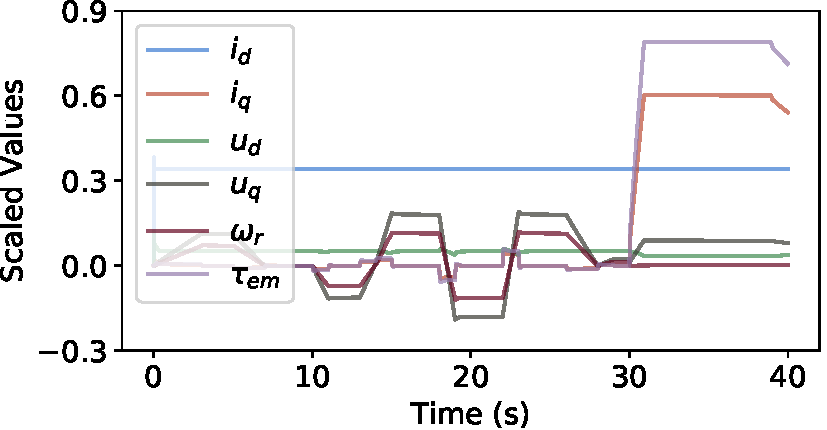
\includegraphics[scale=0.26]{sim} &
          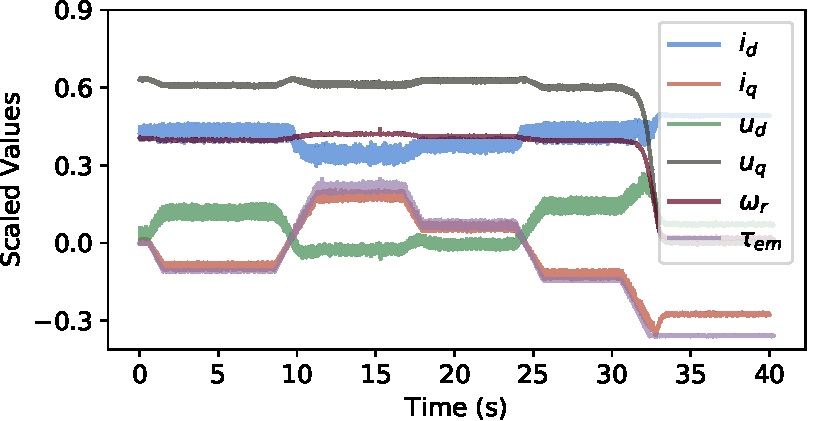
\includegraphics[scale=0.26]{lm45_torquesteps} \\
         \textbf{Simulated sample} &
         \textbf{Real world sample} \\
         \end{tabular}
     \end{center}

 }

 %%%%%%%%%%%%%%%%%%%%%%%%%%%%%%%%%%%%%%%%%%%%%%%%%%%%%%%%%%%%%%%%%%%%%%%%%%%%%%
   \headerbox{Related Work}{name=relatedwork,column=0,below=contributions, span=1}{
 %%%%%%%%%%%%%%%%%%%%%%%%%%%%%%%%%%%%%%%%%%%%%%%%%%%%%%%%%%%%%%%%%%%%%%%%%%%%%%
  \begin{small}
   \begin{itemize}
    \item Physics of electrical motors and controller design \cite{Sylvester1987,Siskind1978cpts}.
    % \item Urban Change Detection in SAR Images by Interactive Learning \cite{saux2013}.
    \item State space model of an induction motor \cite{jadot2009induct}.
    \item Electrical motor dynamics modeling using analytical mechanics \cite{jebai2014cdc}.
    \item Competitive performance of CNNs on sequential tasks \cite{bai2018arxiv}.
    \item Independent Recurrent Neural Network \cite{li2018indrnn}.
   \end{itemize}
   \end{small}
 }

 %%%%%%%%%%%%%%%%%%%%%%%%%%%%%%%%%%%%%%%%%%%%%%%%%%%%%%%%%%%%%%%%%%%%%%%%%%%%%%
   \headerbox{Dataset}{name=dataset,column=0,below=relatedwork, span=1}{
 %%%%%%%%%%%%%%%%%%%%%%%%%%%%%%%%%%%%%%%%%%%%%%%%%%%%%%%%%%%%%%%%%%%%%%%%%%%%%%
 \begin{small}
   \begin{itemize}
      \item 4 kW induction motor
      \item Acquisition rate: 250 Hz
      \item 7 quantities: $i_d, i_q, u_d, u_q, \omega_r, \omega_s, \tau_{em}$
      \item Simulated data: 100 hours, training: 70\% and validation: 30\%
      \item Raw data: 1207 seconds, no $\omega_s$, 10 operating conditions, training: 20\%, and testing: 80\%
   \end{itemize}
   \end{small}
 }

 %%%%%%%%%%%%%%%%%%%%%%%%%%%%%%%%%%%%%%%%%%%%%%%%%%%%%%%%%%%%%%%%%%%%%%%%%%%%%%
   \headerbox{Proposed Architecture}{name=architecture,column=1,row=0,span=2}{
 %%%%%%%%%%%%%%%%%%%%%%%%%%%%%%%%%%%%%%%%%%%%%%%%%%%%%%%%%%%%%%%%%%%%%%%%%%%%%%

 \begin{center}
      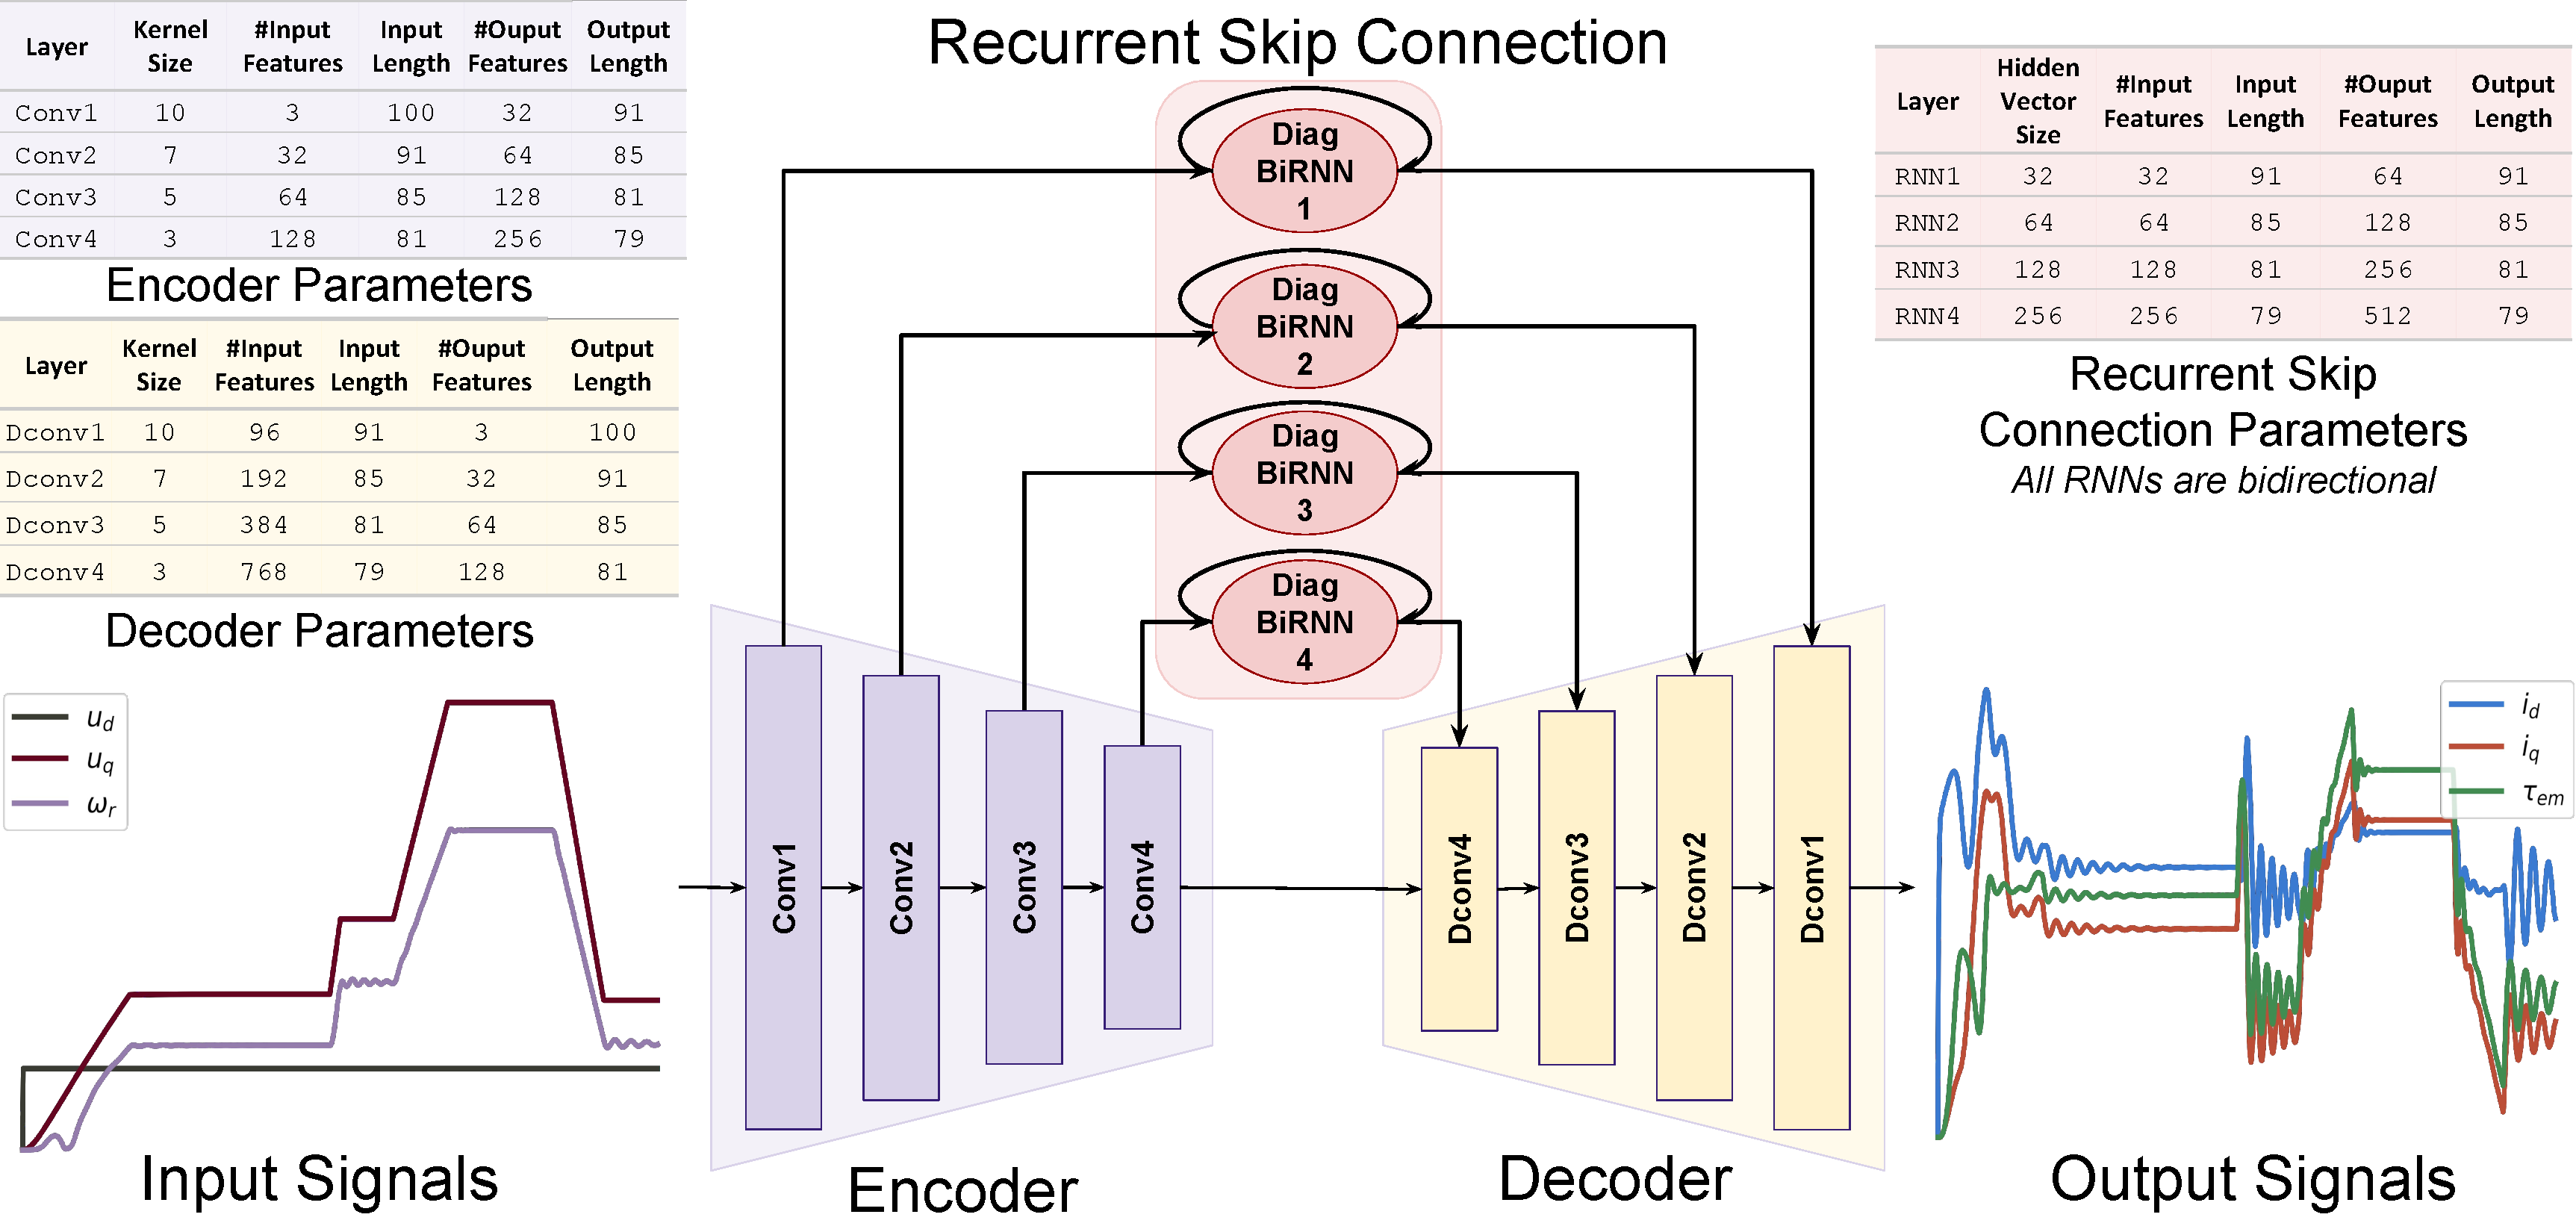
\includegraphics[scale=0.22]{encoder_decoder}
  \end{center}

 }

 %%%%%%%%%%%%%%%%%%%%%%%%%%%%%%%%%%%%%%%%%%%%%%%%%%%%%%%%%%%%%%%%%%%%%%%%%%%%%%
   \headerbox{Results}{name=results,column=1,below=architecture,span=2}{
 %%%%%%%%%%%%%%%%%%%%%%%%%%%%%%%%%%%%%%%%%%%%%%%%%%%%%%%%%%%%%%%%%%%%%%%%%%%%%%
 \setlength{\tabcolsep}{8pt}

  \begin{center}

  \begin{tabular}{c c c c c c}
      \toprule
        \textbf{Model} & \textbf{Window Size} & \textbf{Parameters} &  \textbf{MAE} & \textbf{SMAPE} & \boldmath{$R^2$} \\
       \midrule
       \textbf{Feed-Forward} & 20 & 1118209 & 78.91 & 8.53\% & -0.39 \\
       \textbf{RNN} & 150 & 12001 & 78.26 & 7.76\% & -0.35 \\
       \textbf{LSTM} & 100 & 21889 & 79.58 & 6.29\% & -0.11 \\
       \textbf{CNN} & 100 & 650049 & 79.69 & 6.13\% & -0.14 \\
       \midrule
       \textbf{Encoder-Decoder} & 100  &  1096385 & 81.21 & 4.57\% & 0.29 \\
       \textbf{Skip} & 100  &  364801 & 28.96 & 3.71\% & 0.42 \\
       \textbf{RNN-Skip} & 100  &  638145 & 28.18 & 3.42\% & 0.43 \\
       \textbf{BiRNN-Skip} & 100  &  967105 & 27.96 & 3.31\% & 0.41 \\
       \textbf{DiagBiRNN-Skip} & 100  &  618465 & \textbf{26.88} & \textbf{1.09}\% & \textbf{0.95} \\
       \bottomrule
    \end{tabular}
    \\
    Results for the benchmark and the proposed model variants obtained on the simulated validation set.
    \vspace{0.5em}

    \begin{tabular}{c c c}
       \stackunder[2.5pt]{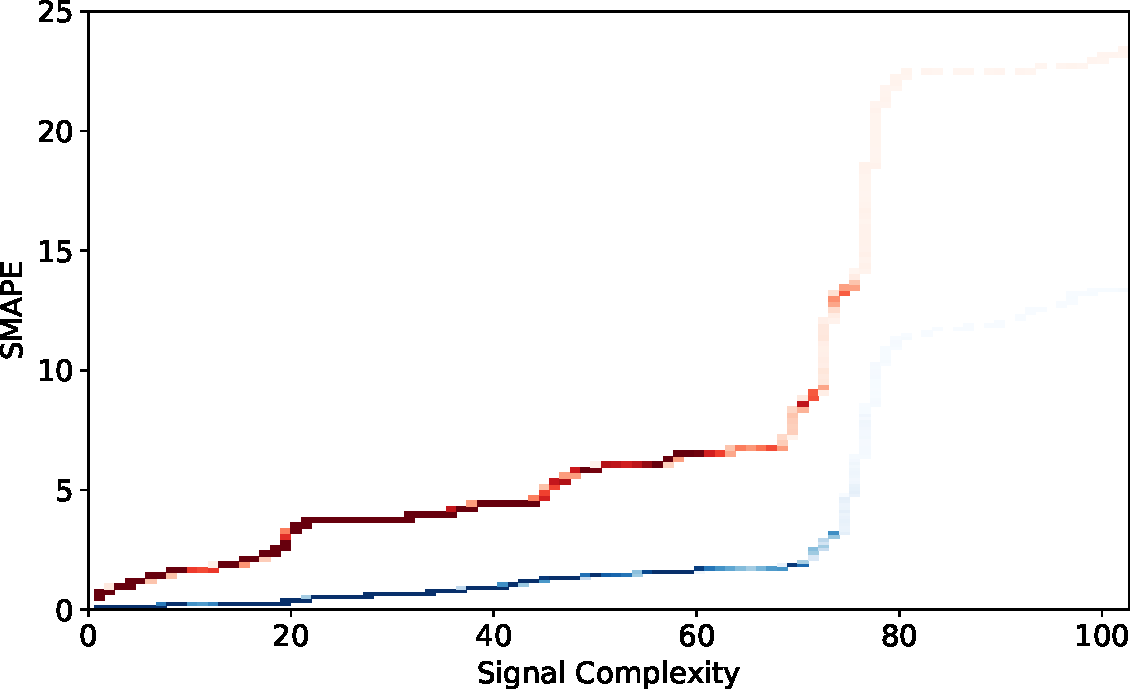
\includegraphics[scale=0.23]{sc_smape_curr1.pdf}}{(a) Current $i_d$}
     \llap{\shiftleft{4.0cm}{\raisebox{2.0cm}{%  move next graphics to top right corner
     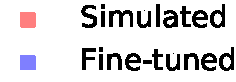
\includegraphics[scale=0.35]{legend.pdf}%
       }}}
     \stackunder[2.5pt]{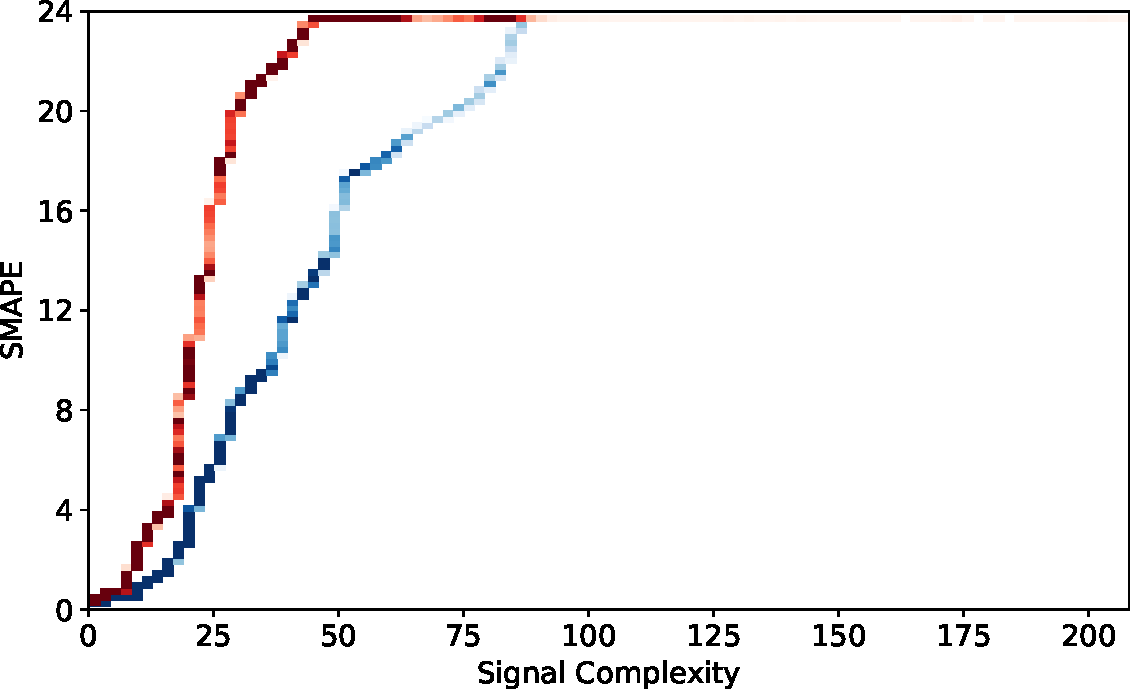
\includegraphics[scale=0.23]{sc_smape_curr2.pdf}}{(b) Current $i_q$}
     \llap{\shiftleft{2.0cm}{\raisebox{1.0cm}{%  move next graphics to top right corner
     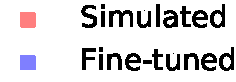
\includegraphics[scale=0.35]{legend.pdf}%
       }}}
     \stackunder[2.5pt]{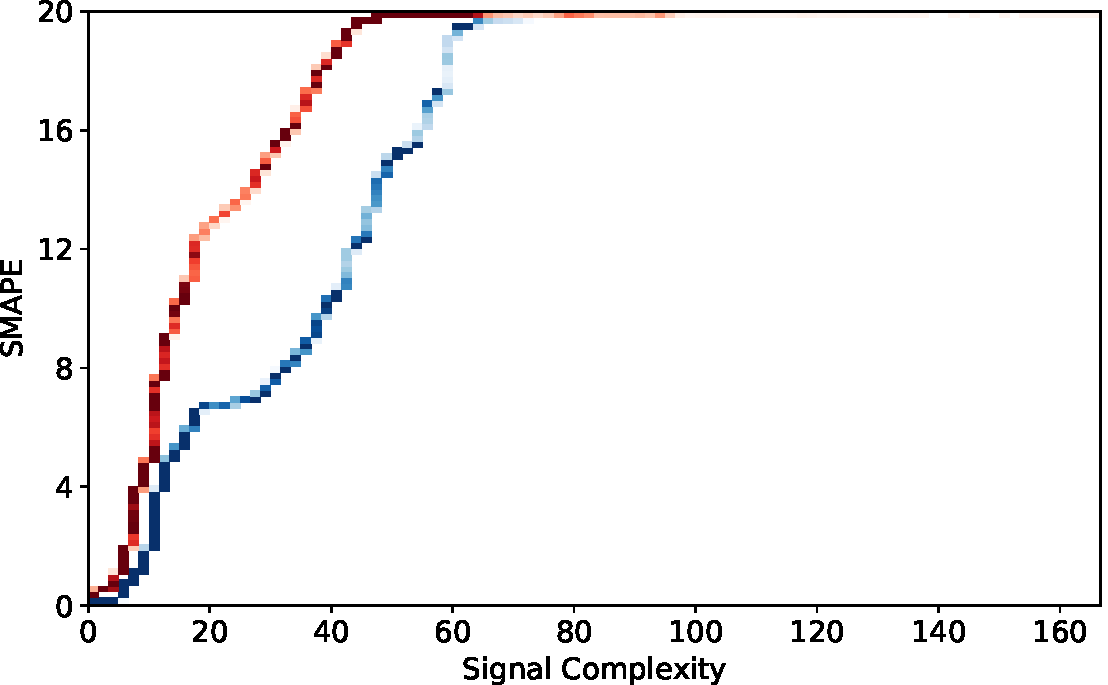
\includegraphics[scale=0.23]{sc_smape_torque.pdf}}{(c) Torque $\tau_{em}$}
      \llap{\shiftleft{2.0cm}{\raisebox{1.0cm}{%  move next graphics to top right corner
     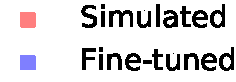
\includegraphics[scale=0.35]{legend.pdf}%
       }}}

       \end{tabular}
       \\
       Comparison of simulated and fine-tuned model using SMAPE vs Signal Complexity(Total Variation) graph. \\
       \vspace{0.5em}


    \begin{tabular}{c c c}
    \stackunder[2.5pt]{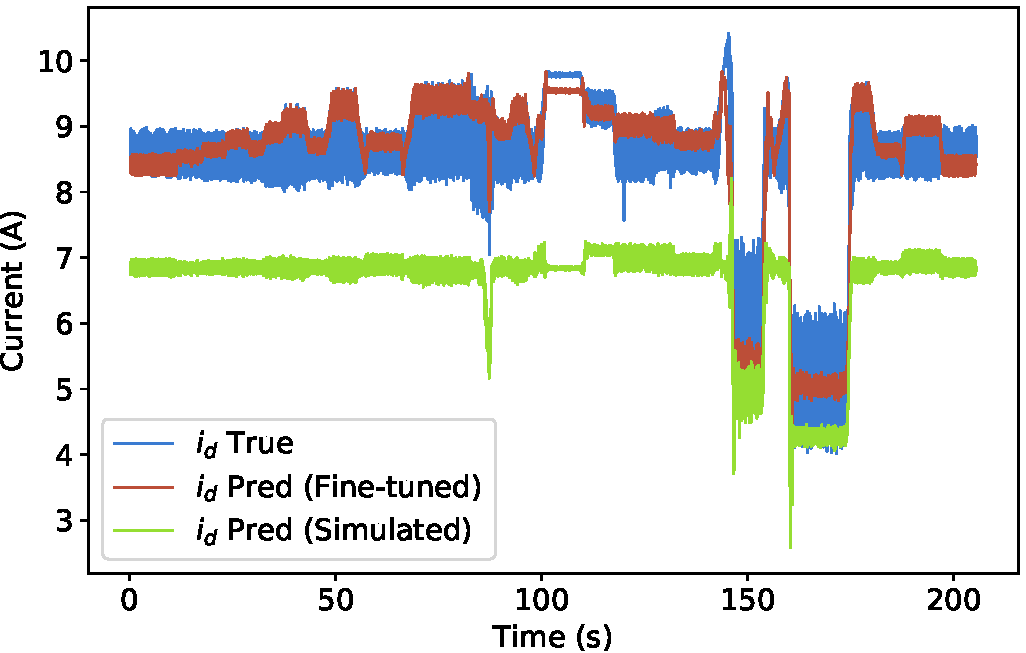
\includegraphics[scale=0.25]{res_sim_curr1.pdf}}{(a) Current $i_d$} &
      \stackunder[2.5pt]{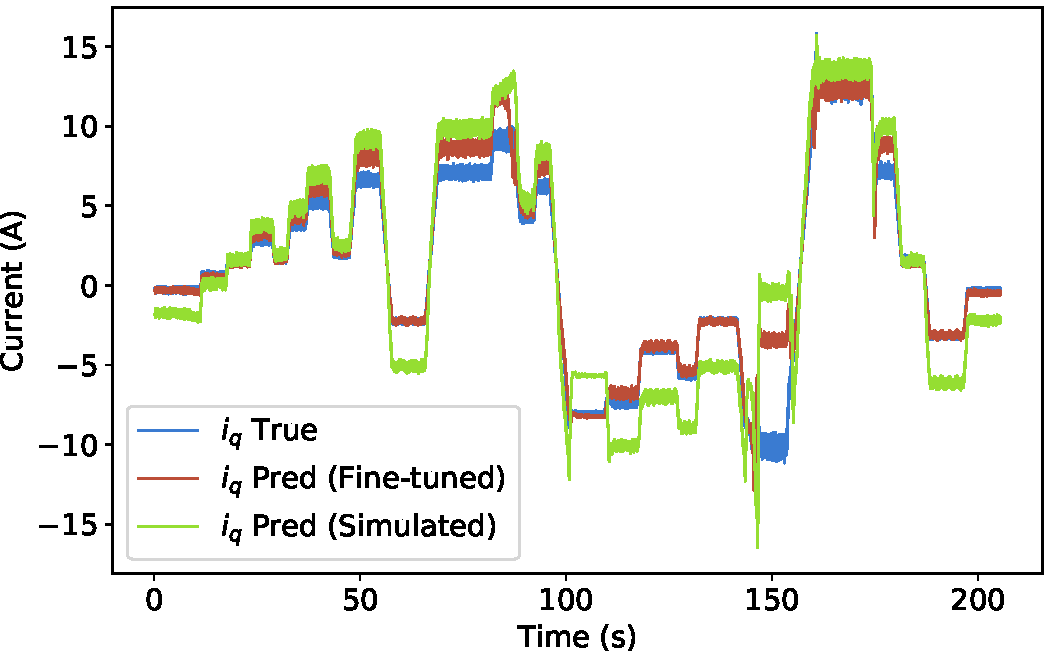
\includegraphics[scale=0.25]{res_sim_curr2.pdf}}{(b) Current $i_q$} &
      \stackunder[2.5pt]{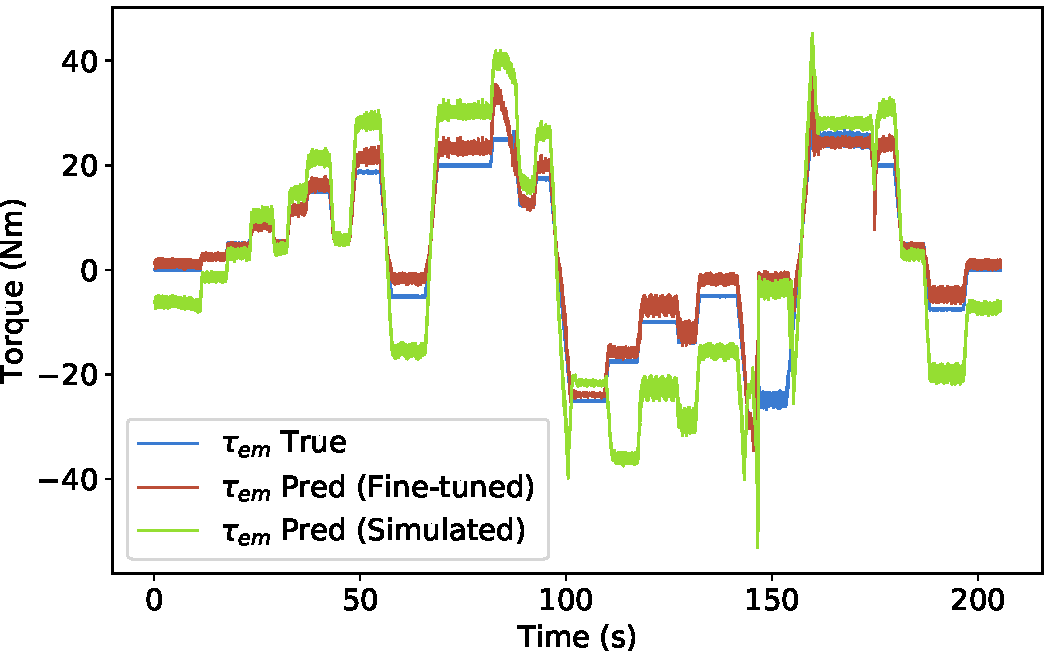
\includegraphics[scale=0.25]{res_sim_torque.pdf}}{(c) Torque $\tau_{em}$}
    \end{tabular}
      Predicted result of one of the experiments from the test set.

    \end{center}
 }

  %%%%%%%%%%%%%%%%%%%%%%%%%%%%%%%%%%%%%%%%%%%%%%%%%%%%%%%%%%%%%%%%%%%%%%%%%%%%%%
    \headerbox{Contributions}{name=contrib,column=3,row=0}{
  %%%%%%%%%%%%%%%%%%%%%%%%%%%%%%%%%%%%%%%%%%%%%%%%%%%%%%%%%%%%%%%%%%%%%%%%%%%%%%
          \begin{center}
  \centering
  \begin{itemize}
    \item New \textit{Encoder-Decoder architecture} with \textit{diagonalized recurrent skip connection} to effectively learn time-series relationship between different electrical quantities.
      \begin{footnotesize}
      \begin{align*}
          h_t = \text{tanh}(w \odot x_t + u \odot h_{t-1} + b)
      \end{align*}
      \end{footnotesize}
      \begin{small}
      where $w \in \mathbb{R}^M$, $u \in \mathbb{R}^M$, and $b \in \mathbb{R}^M$ are input weights.
      \end{small}

    \item A novel \textit{loss function} that uses fast variations present in the electrical motor signals to avoid model bias.
    \begin{footnotesize}
    \begin{align*}
     \mathcal{L}_{\tiny{\text{TV-MSE}}} = \frac{1}{N}\sum_{i=1}^{N}\underbrace{\left(\sum_{t=1}^{T-1} |y^i_t - y^i_{t+1}|\right)}_\textrm{Total Variation} \overbrace{\left(\frac{1}{T}\sum^{T}_{t=1}(y^i_t - \hat{y^i_t})^2 \right)}^\textrm{MSE}
    \end{align*}
    \end{footnotesize}
    \begin{small}
    where $y^i_t$ and $\hat{y^i_t}$ are the values of output and predicted sample $i$ at time-step $t$, respectively. $N$ is the number of training samples, where each sample is of duration $T$.
    \end{small}

    \item \textit{Two datasets}; a large dataset of simulated electrical motor operations and a small dataset of sensor data recorded from the real-world operations of electrical motors.
    % \item We analyse the capability of the proposed method by using a new analysis technique and we demonstrate the transfer learning capability of our approach.
    \end{itemize}

  \end{center}

\begin{center}
\fboxsep0pt
\colorbox{light-gray1}{\begin{minipage}{6.2cm}
\qrcode{qr.png}{smartphone.png}{
Visit project page for\\
full paper, code, and dataset
}
\end{minipage}}
\end{center}

    }



 % %%%%%%%%%%%%%%%%%%%%%%%%%%%%%%%%%%%%%%%%%%%%%%%%%%%%%%%%%%%%%%%%%%%%%%%%%%%%%%
 %   \headerbox{}{name=results2,column=3,row=0}{
 % %%%%%%%%%%%%%%%%%%%%%%%%%%%%%%%%%%%%%%%%%%%%%%%%%%%%%%%%%%%%%%%%%%%%%%%%%%%%%%
 %         \begin{center}
 %
 %
 %         \end{center}
 %
 %   \footnotesize\textbf{Top and bottom of each subfigure shows predicted and ground truth sequence respectively.}
 %
 %   }


  %%%%%%%%%%%%%%%%%%%%%%%%%%%%%%%%%%%%%%%%%%%%%%%%%%%%%%%%%%%%%%%%%%%%%%%%%%%%%%
    \headerbox{References}{name=references,column=3,below=contrib}{
  %%%%%%%%%%%%%%%%%%%%%%%%%%%%%%%%%%%%%%%%%%%%%%%%%%%%%%%%%%%%%%%%%%%%%%%%%%%%%%


     \bibliographystyle{IEEEbib}
      \tiny\bibliography{ref}

    }

    %%%%%%%%%%%%%%%%%%%%%%%%%%%%%%%%%%%%%%%%%%%%%%%%%%%%%%%%%%%%%%%%%%%%%%%%%%%%%%
      \headerbox{Affiliations}{name=ack,column=3,below=references,above=bottom}{
    %%%%%%%%%%%%%%%%%%%%%%%%%%%%%%%%%%%%%%%%%%%%%%%%%%%%%%%%%%%%%%%%%%%%%%%%%%%%%%


    \begin{tiny}
    {\raggedleft
      \textsuperscript{1} Universit\'{e} Paris-Saclay, CentraleSup\'{e}lec, Inria, Centre de Vision Num\'{e}rique, 91190, Gif-sur-Yvette, France \\
      \textsuperscript{2} Schneider Toshiba Inverter Europe, 33, Rue Andr\'e Blanchet, 27120, Pacy-sur-Eure, France \\
      \textsuperscript{3} Samovar, CNRS, T\'{e}l\'{e}com SudParis, Institut Polytechnique de Paris, \\
            9, Rue Charles Fourier, 91011, Evry Cedex, France \\
    }
    \end{tiny}

    }




\end{poster}%
%
\end{document}
